\documentclass[12pt,a4paper]{article}
\usepackage[T1]{fontenc}
\usepackage[a4paper]{geometry}
\usepackage[portuges,brazilian]{babel}
\usepackage[utf8]{inputenc}
\usepackage{setspace}
\usepackage{libertine}
\usepackage{graphicx}	
\usepackage{ragged2e} 	
\usepackage{hyperref}	

\begin{document} 
\begin{figure}
    \flushright
    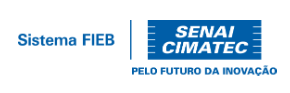
\includegraphics[scale=0.5]{Logo_senai.png}
\end{figure}

\title{Robótica no auxílio de pessoas com deficiências físicas.}
\author{Jean Paulo Silva\thanks{jean.silva@fbter.org.br SENAI-CIMATEC  CCRoSA- Centro de Competência em Robótica e Sistemas Autônomos.}}
 
 

    \maketitle
    \pagenumbering{arabic}
    \singlespacing


    \textbf{AUDIÊNCIA}

    \par Esta palestra tem como público-alvo estudantes universitários e pesquisadores das áreas de automação, robótica e saúde. A apresentação foca em introduzir a relação entre as áreas baseando-se em novas tecnologias para o auxílio de pessoas com deficiências físicas.
    \newline
    \newline
    \par \textbf{TEMPO}
    \par O tempo total de apresentação é de 20 minutos. Esse tempo será distribuido entre as partes da apresentação:
    \begin{itemize}
    \item Introdução;
    \item Contexto;
    \item Definições;
    \item Exemplos;
    \item Conclusão.
    \end{itemize}
    \par A apresentação será feita em sequência de slides utilizando a ferramenta LaTeX. Seguirei um padrão de 1 minuto e 30 segundos por slide durante as partes de introdução, contexto e conclusão. As partes de contexto e exemplo podem apresentar vídeos ou explicações mais extensivas por slides. Neste caso, o número de slides será reduzido para que toda a apresentação caiba nos 20 minutos.
    \newline
    \newline
    \par \textbf{PERFIL}
    \par A imagem que eu quero passar é de uma pessoa que aprendeu um assunto e está animado para conversar esse assunto com a maior quantidade de pessoas possível, mesmo que tenha que passar um tempo explicando tal assunto. Isso se traduz por uma não-formalidade na fala e trazer o máximo de exemplos possíveis na apresentação. A imagem também pode ser traduzida por roupas e plano de fundo brancos, para lembrar o tema de saúde.
    \newline
    \newline
    \par \textbf{CONTEXTO}
    \par O tema está inserido nas áreas de robótica e fisioterapia, com grandes ênfases na criação de próteses e do retorno da movimentação e sensibilidade de partes do corpo de pacientes.
    \par Na sociedade atual, mais de um milhão de amputações de membros são causadas devido à acidentes, doenças cardiovasculares, tumores e doenças congênitas \cite{5}.
    \par A saúde é uma das áreas que mais se beneficiou com os avanços tecnológicos recentes. No campo da fisioterapia, o destaque fica por conta da utilização de recursos robóticos auxiliares ao tratamento \cite{1}.
    \par Um dos exemplos que mais chamou atenção da mídia foi o caso Les Baugh (figura \ref{fig:les}), um homem de 40 anos que perdeu os dois braços em um acidente elétrico. Ele participou de um estudo pela universidade Johns Hopkins em que ele podia controlar duas próteses robóticas depois de uma cirurgia de reinervação das partes necessárias para o experimento.
    \begin{figure}[ht]
        \caption{Les Baugh, utilizando duas próteses robóticas. \cite{6}}
        \centering
        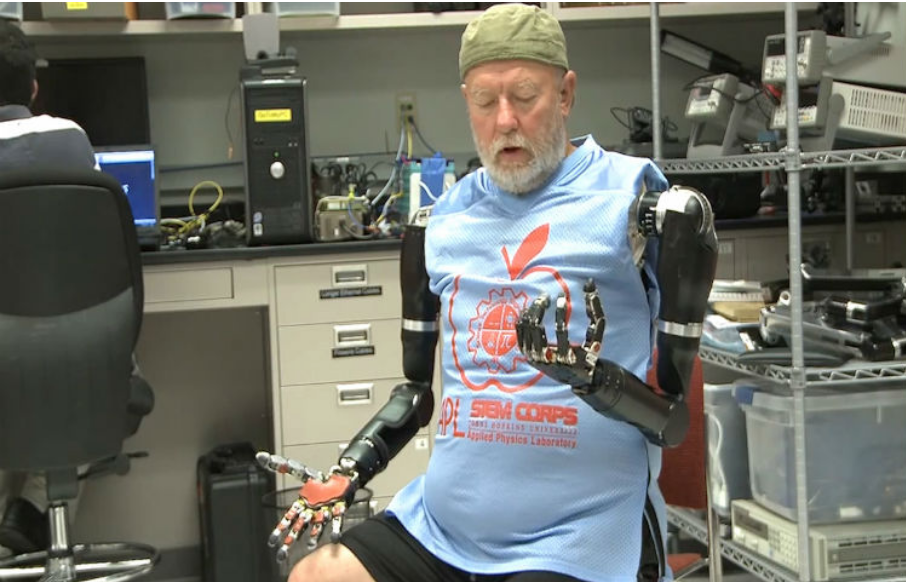
\includegraphics[width=0.6\linewidth]
        {images/Les.png}
        \label{fig:les}
    \end{figure}
    \par Uma das importantes abordagens de reabilitação, especialmente para recuperar a função motora, é a fisioterapia incluindo práticas repetitivas e intensas. Várias modalidades de reabilitação são utilizadas, e em sua grande maioria com dispositivos auxiliares \cite{2}.
    \par Uma das ferramentas é o aparelho Erigo (como mostra a figura \ref{fig:erigo}). É um exoesqueleto que ajuda pacientes internados em UTI que requerem início imediato de tratamento por danos neurológicos, mas também pode realizar tratamentos cardiovasculares pela sua capacidade de estabilizar como cama horizontal ou vertical \cite{4}.
    \begin{figure}[ht]
        \caption{Solução Erigo, Hocoma. \cite{4}}
        \centering
        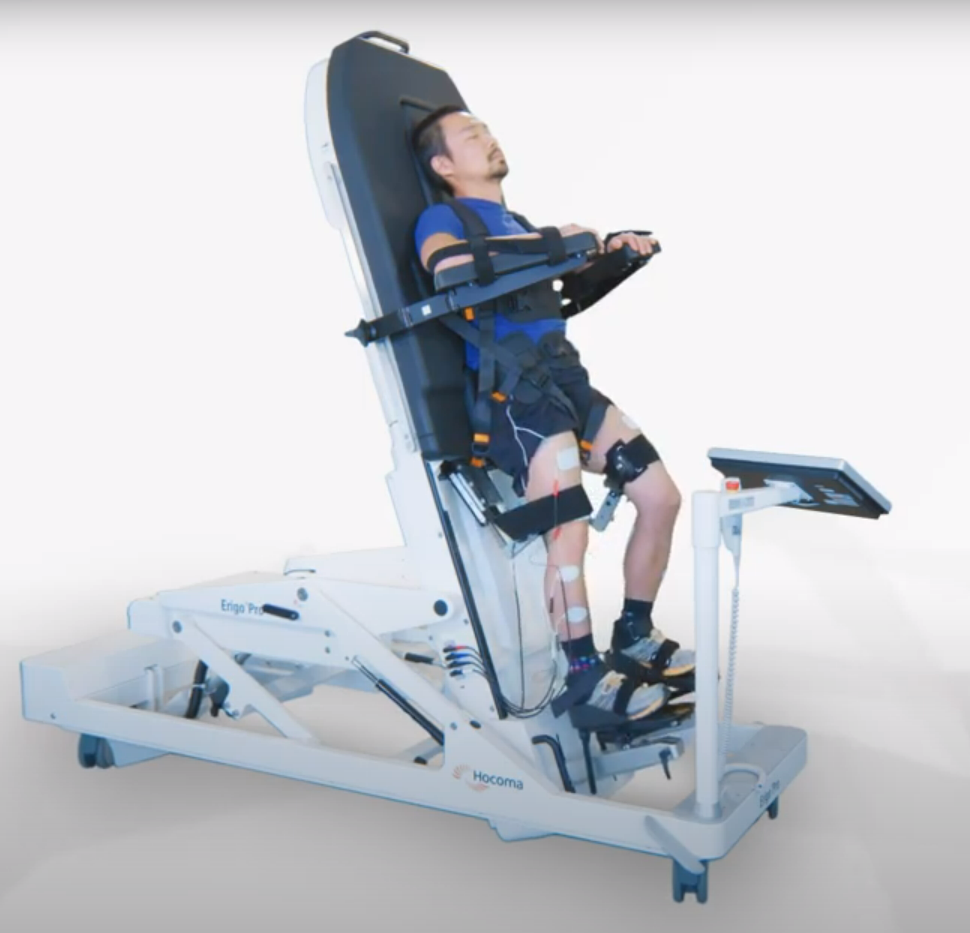
\includegraphics[width=0.6\linewidth]
        {images/erigo.png}
        \label{fig:erigo}
    \end{figure}

    \par Outra metodologia em estudo é a marcha robótica para o tratamento de pessoas com lesões na medula \cite{1} \cite{3}, figura \ref{fig:marcha}.


    \begin{figure}[ht]
        \caption{Marcha Robótica. Fonte: ISTOÉ - Canal no Youtube. \cite{3}}
        \centering
        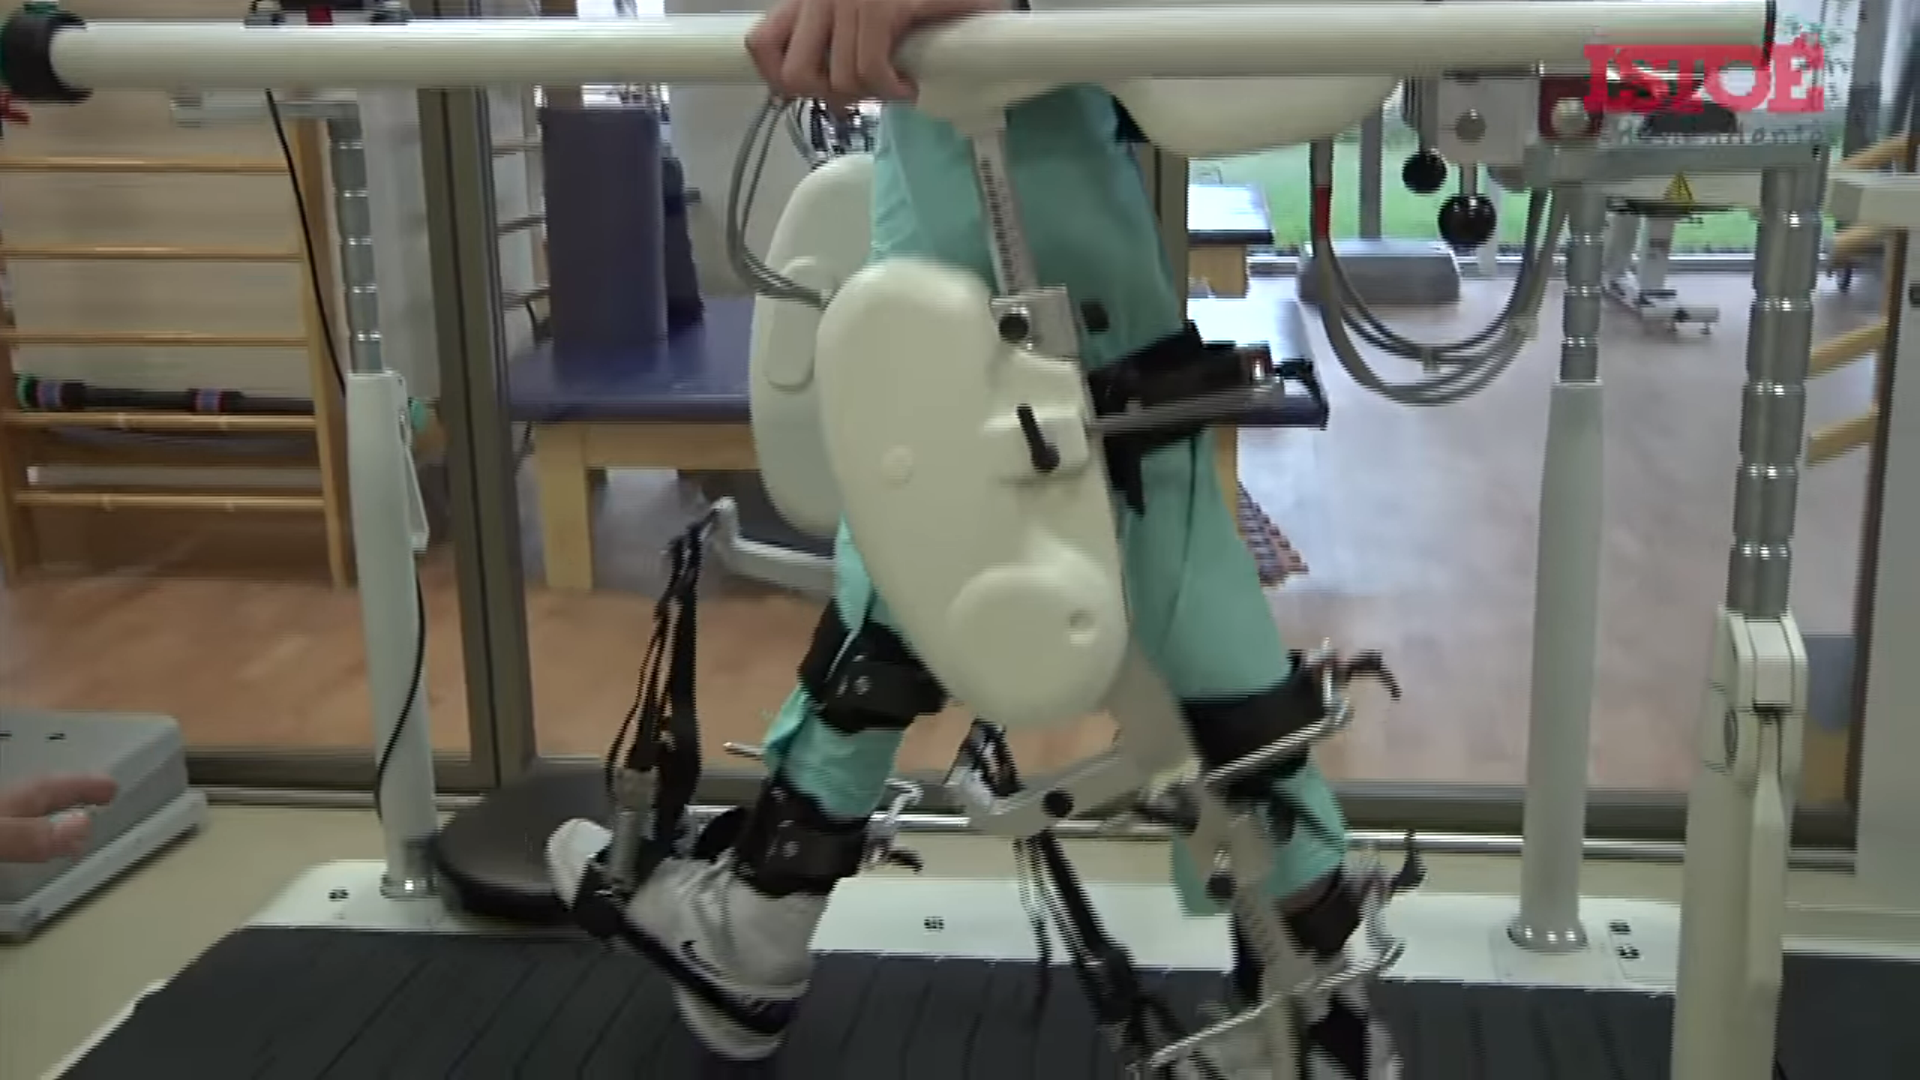
\includegraphics[width=0.6\linewidth]
        {images/marcha.png}
        \label{fig:marcha}
    \end{figure}
    

    \par A apresentação tem o intuito de demonstrar novas tecnologias, suas metodologias, resultados e aplicações na área da robótica e fisioterapia em conjunto.
    \par Vale também ressaltar que as novas tecnologias tem foco na ajuda do profissional da saúde. Essas tecnologias necessitam de uma supervisão para a eficiência da reabilitação do paciente.
    \newpage
    \newpage
    \begin{thebibliography}{BIBLIOGRAFIA}
 
        \bibitem{1} SECAD. \textbf{Fisioterapia e Robótica: complemento às técnicas de reabilitação}. Disponível em: \url{https://www.secad.com.br/blog/fisioterapia/reabilitacao-com-fisioterapia-e-robotica/}
        \bibitem{2} SOUZA, Francine Bertolais do Valle. \textbf{Benefícios da marcha com assistência robótica na lesão medular: uma revisão sistemática.}
        \bibitem{3} Revista ISTOÉ. \textbf{Fisioterapia Robótica} Disponível em: \url{https://www.youtube.com/watch?v=GL_9nyWuXc0}
        \bibitem{4} Hocoma. \textbf{Erigo}. Disponível em: \url{https://www.hocoma.com/solutions/erigo/}
        \bibitem{5} GOPURA, Ruwan. \textbf{Robotic Prosthetic Limbs.}
        \bibitem{6} NUNES, Natalia. \textbf{Paciente amputado controla duas próteses robóticas com o cérebro.} Disponível em: \url{https://saudebusiness.com/hospital/paciente-amputado-controle-duas-proteses-roboticas-com-o-cerebro/}
    \end{thebibliography}


\end{document}